\documentclass[../main.tex]{subfiles}

\graphicspath{{\subfix{../figures/}}}

\begin{document}

\Gls{spa} refers to a \gls{cryoem} technique that allows to obtain models of proteins at almost atomic resolution. Although it has been around for decades, recent technological leaps have led to an increase in interest from users and researchers. This technique involves everything from the sample preparation to the final image processing, including the image acquisition at the microscope\cite{dimitry2019}. However, this chapter will focus on explaining the image processing part of the workflow.

The essence of \gls{spa} lies on rapidly freezing thousands of specimens in a thin film of ice. In this way, each specimen will be held in place with the random orientation it had before it was frozen. At this point, the sample is scanned by a \gls{tem}, obtaining 2D projections of the specimens. These projections can be thought of as a shadow of the electron density of the sample. Using advanced image processing techniques, this collection of projections can be used to reconstruct the 3D electron density map of the specimen under study. Figure \ref{fig:2:acquisition_reconstruction} provides an illustration of this process. Nevertheless, the reconstruction process involves several challenges, as the input images have very poor \gls{snr} and other artefacts.

\begin{figure}[htbp]
    \centering
    \begin{subfigure}[b]{0.45\textwidth}
         \centering
         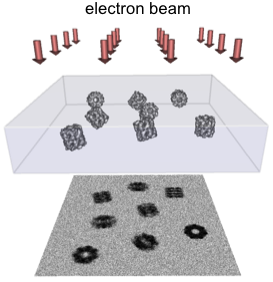
\includegraphics[width=\textwidth]{SPA/projection_reconstruction/acquisition}
         \caption{Image acquisition}
         \label{fig:2:projection_reconstruction:acquisition}
    \end{subfigure}
    \hfill
    \begin{subfigure}[b]{0.45\textwidth}
         \centering
         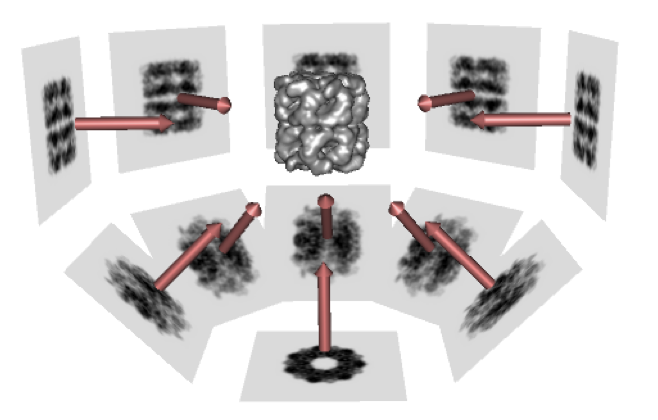
\includegraphics[width=\textwidth]{SPA/projection_reconstruction/reconstruction}
         \caption{Reconstruction}
         \label{fig:2:projection_reconstruction:reconstruction}
    \end{subfigure}\\
    Images obtained from: \cite{greg}
    \caption{Image acquisition and structure reconstruction}
    \label{fig:2:acquisition_reconstruction}
\end{figure}

The studied sample is prepared on a copper of gold grid, which is inserted into the \gls{em} chamber. Each of spot of the sample can only be exposed to the electron beam for a limited amount of time before degradation occurs. Recent leaps in sensor technology have sped up the required exposition time for the sensors, enabling them to capture multiple frames of the sample before degrading it. The set of frames captured from a given spot is known as movie. These movies serve as the starting point of the \gls{spa} image processing workflow. This workflow is summarised in the Figure \ref{fig:2:spa_workflow} and it will be detailed hereafter. 

\begin{landscape}
    \begin{figure}
        \centering
        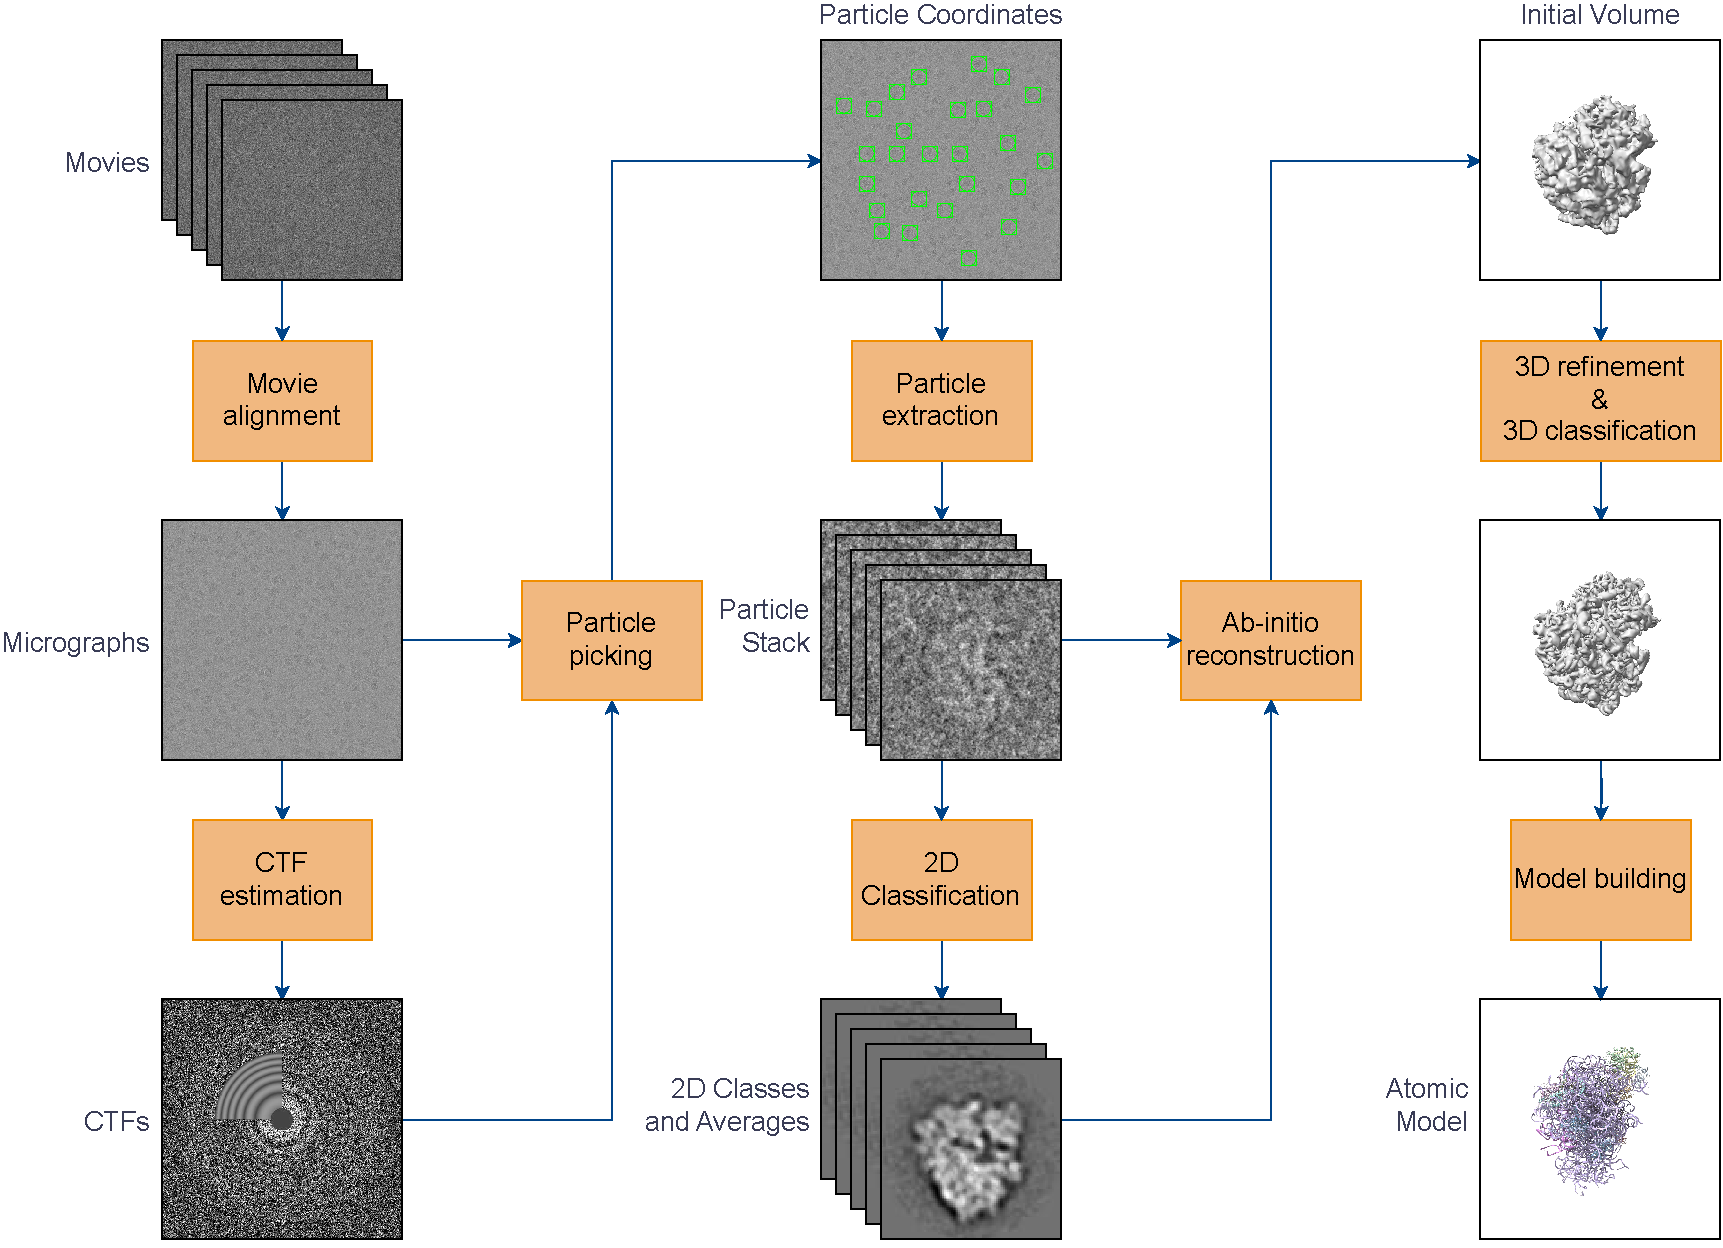
\includegraphics[height=15cm]{SPA/workflow}
        \caption{SPA workflow}
        \label{fig:2:spa_workflow}
    \end{figure}
\end{landscape}

\section{SPA image processing steps}

\subsection{Movie alignment}
In the movie alignment stage all the frames of a movie are averaged into a single image known as micrograph. This helps to increase the \gls{snr}, as the uncorrelated part of the noise tends to cancel out across images. Note that the noise induced by the vitreous ice is the same for all the frames of a given movie so it will not be removed when averaging frames. 

The frames contained in a movie are in chronological order. As a result, the last images have a higher electron dose than the first ones, which translates into a more severe deterioration of their atomic structure  Moreover, this deterioration has a higher influence in the higher frequencies of the image. These facts need to be taken into account when combining all the images, in such a way that the high frequencies of the last images have less weight\cite{cryoem101}. 

Additionally, the electron beam positioning system drifts between frames and the sample tends to bend, which tends to produce optical flow between frames. Consequently, the frames are not aligned to one another. This needs to be fixed before attempting to average the frames, as otherwise the resulting micrograph would loose resolution.

\subsection{CTF estimation}
\Glspl{tem} do not have a planar frequency response. Instead, they ``colour'' the images with a characteristic \gls{ctf} known as Thon rings. This transfer function has a sinusoidal appearance, with decreasing periodicity and a overall tendency to attenuate higher frequencies\cite{cryoem101}.  In addition, the rings may have elliptical shape, being wider in some axis. This is known as astigmatism. A example of a \gls{tem} \gls{ctf} is shown in the Figure \ref{fig:2:ctf}.

\begin{figure}[htbp]
    \centering
    \begin{subfigure}[b]{0.3\textwidth}
        \centering
        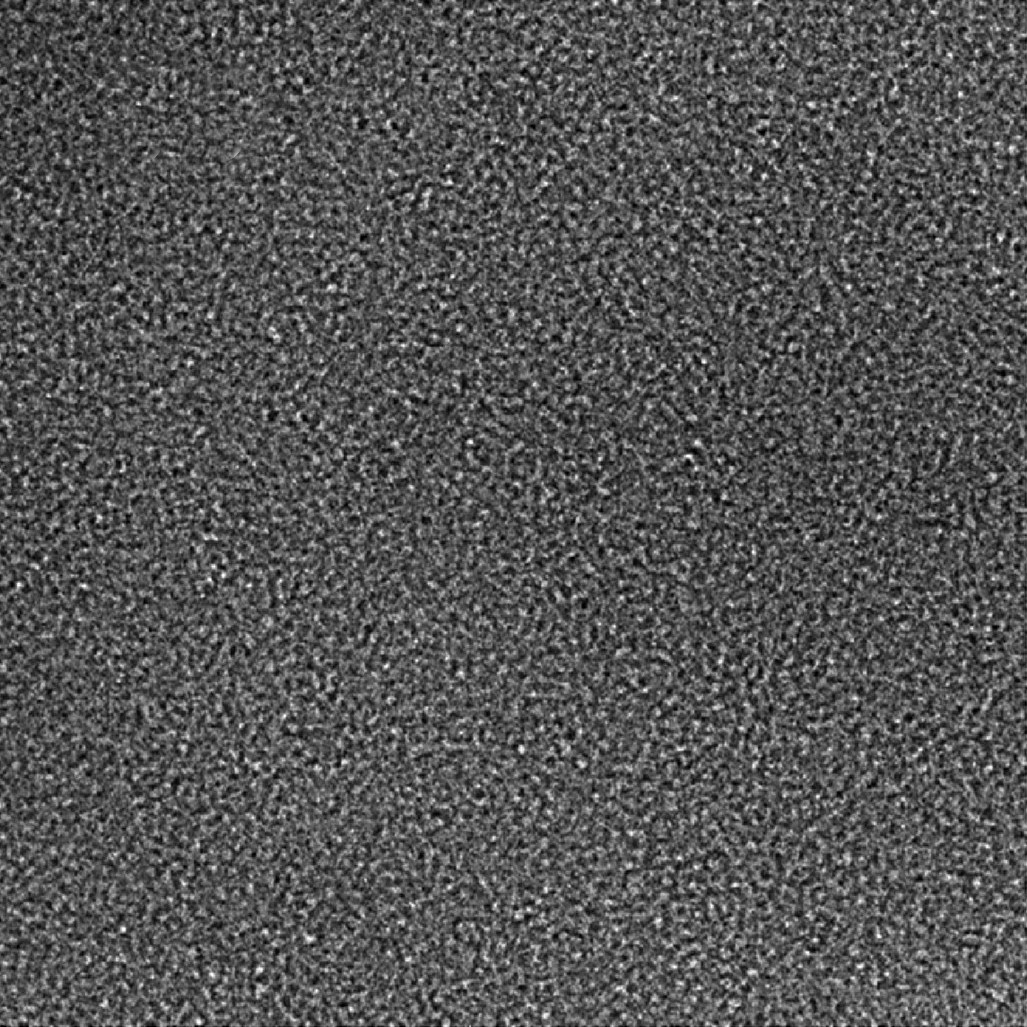
\includegraphics[width=\textwidth]{SPA/ctf/micrograph_0.5}
        \caption{Micrograph with $0.5\si{\micro\metre}$ defocus}
        \label{fig:2:ctf:mic0.5}
    \end{subfigure}
    \hfill
    \begin{subfigure}[b]{0.3\textwidth}
        \centering
        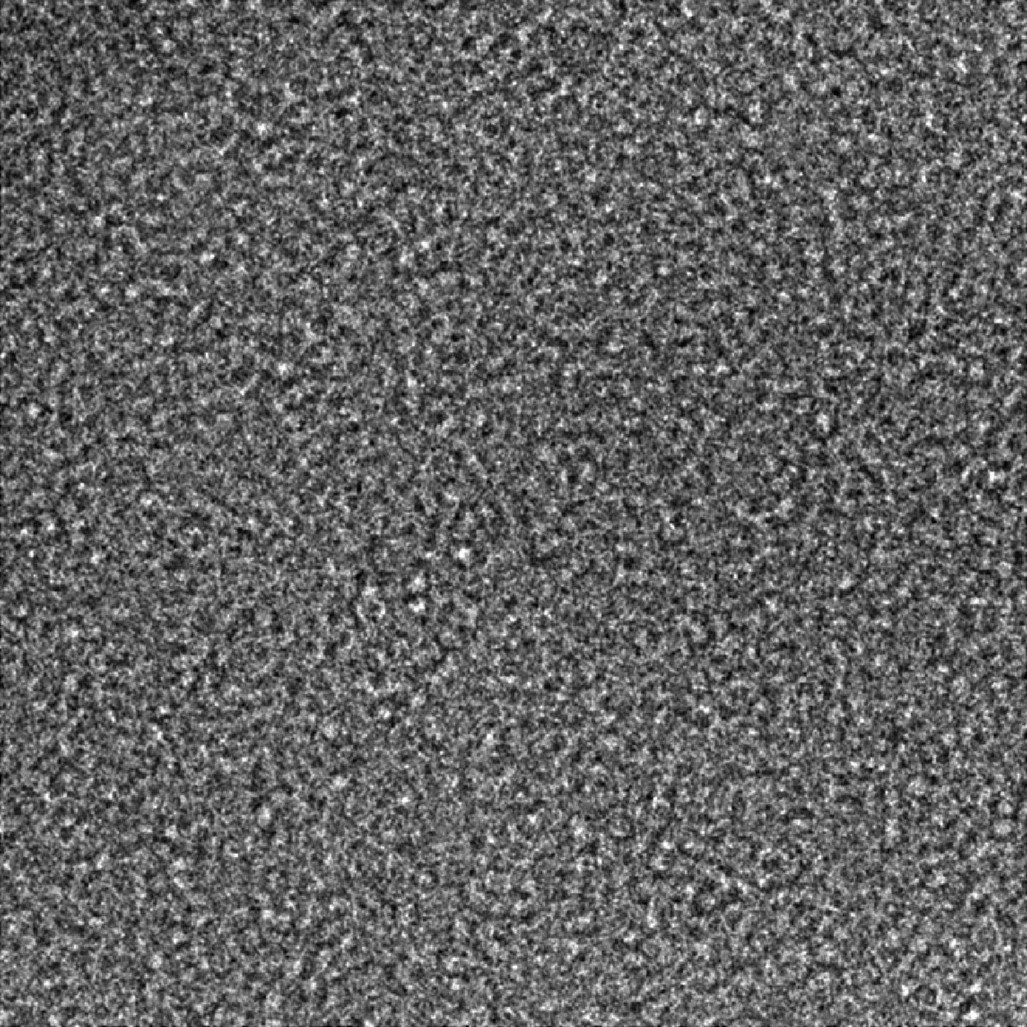
\includegraphics[width=\textwidth]{SPA/ctf/micrograph_1}
        \caption{Micrograph with $1.0\si{\micro\metre}$ defocus}
        \label{fig:2:ctf:mic1.0}
    \end{subfigure}
    \hfill
    \begin{subfigure}[b]{0.3\textwidth}
        \centering
        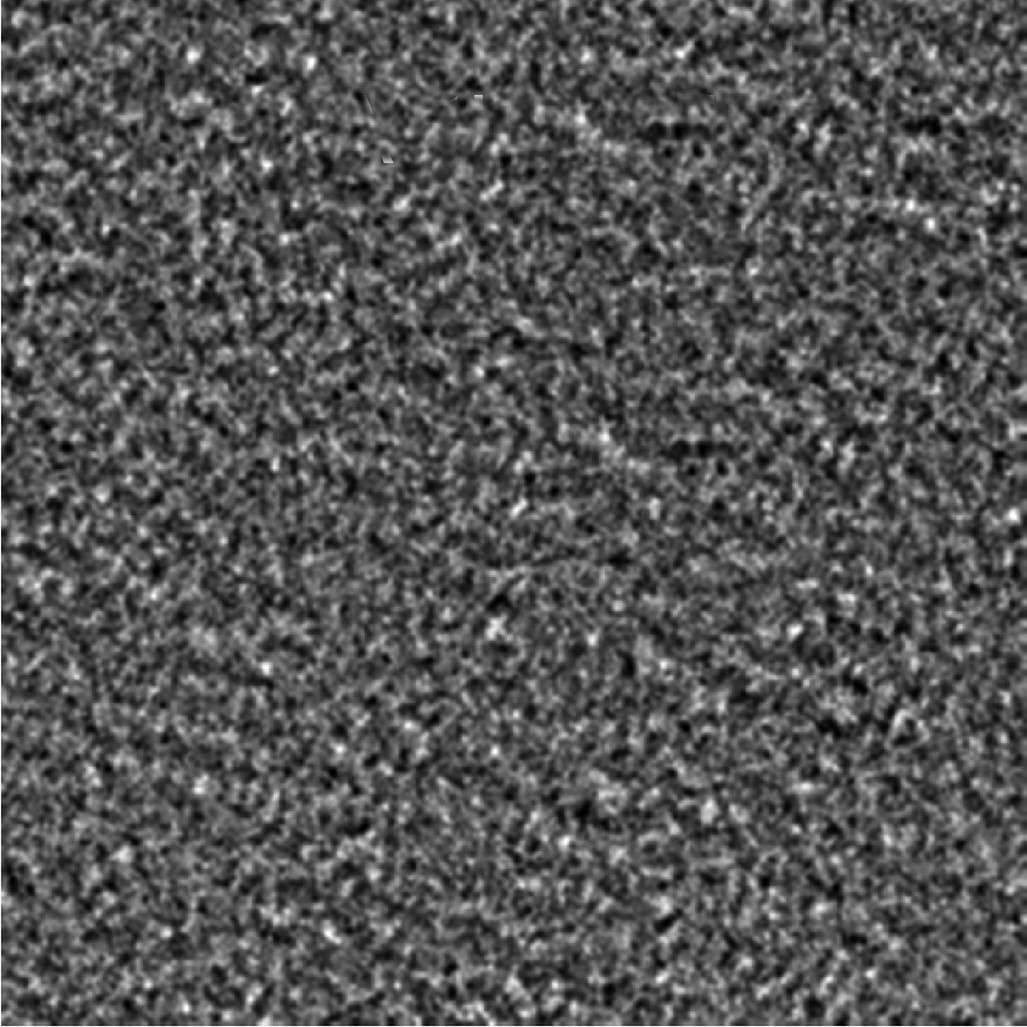
\includegraphics[width=\textwidth]{SPA/ctf/micrograph_as}
        \caption{Micrograph with astigmatism}
        \label{fig:2:ctf:mic_as}
    \end{subfigure}\\
    \vspace{1em}
    \begin{subfigure}[b]{0.3\textwidth}
        \centering
        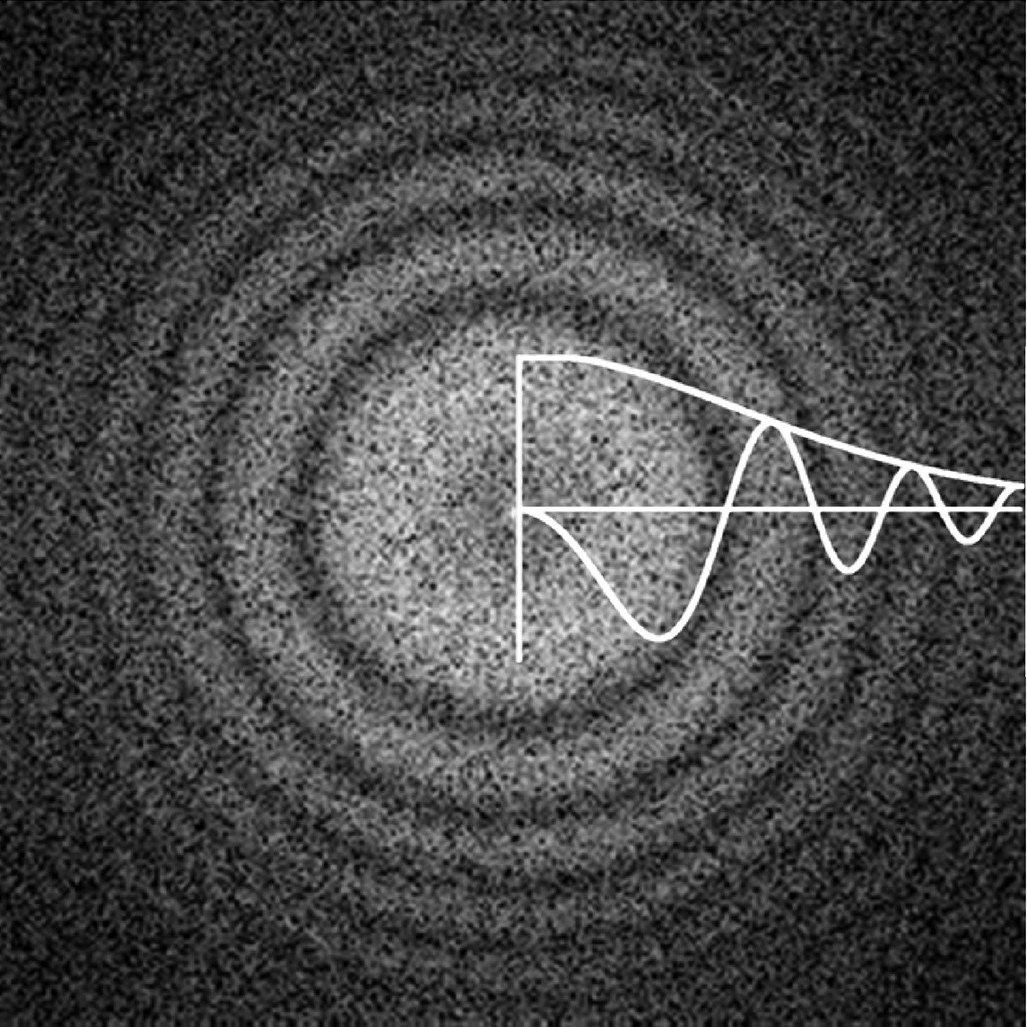
\includegraphics[width=\textwidth]{SPA/ctf/psd_0.5}
        \caption{Micrograph PSD with $0.5\si{\micro\metre}$ defocus}
        \label{fig:2:ctf:psd0.5}
    \end{subfigure}
    \hfill
    \begin{subfigure}[b]{0.3\textwidth}
        \centering
        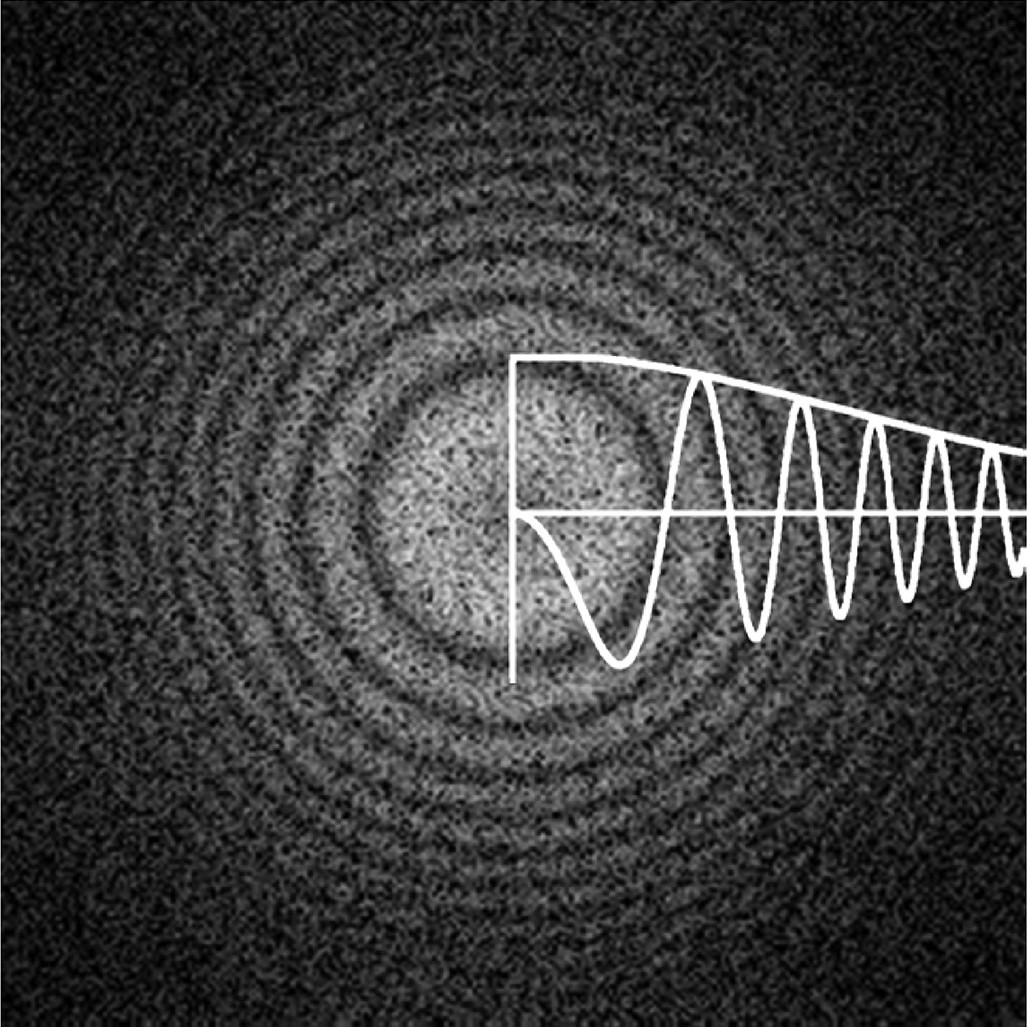
\includegraphics[width=\textwidth]{SPA/ctf/psd_1}
        \caption{Micrograph PSD with $1.0\si{\micro\metre}$ defocus}
        \label{fig:2:ctf:psd1.0}
    \end{subfigure}
    \hfill
    \begin{subfigure}[b]{0.3\textwidth}
        \centering
        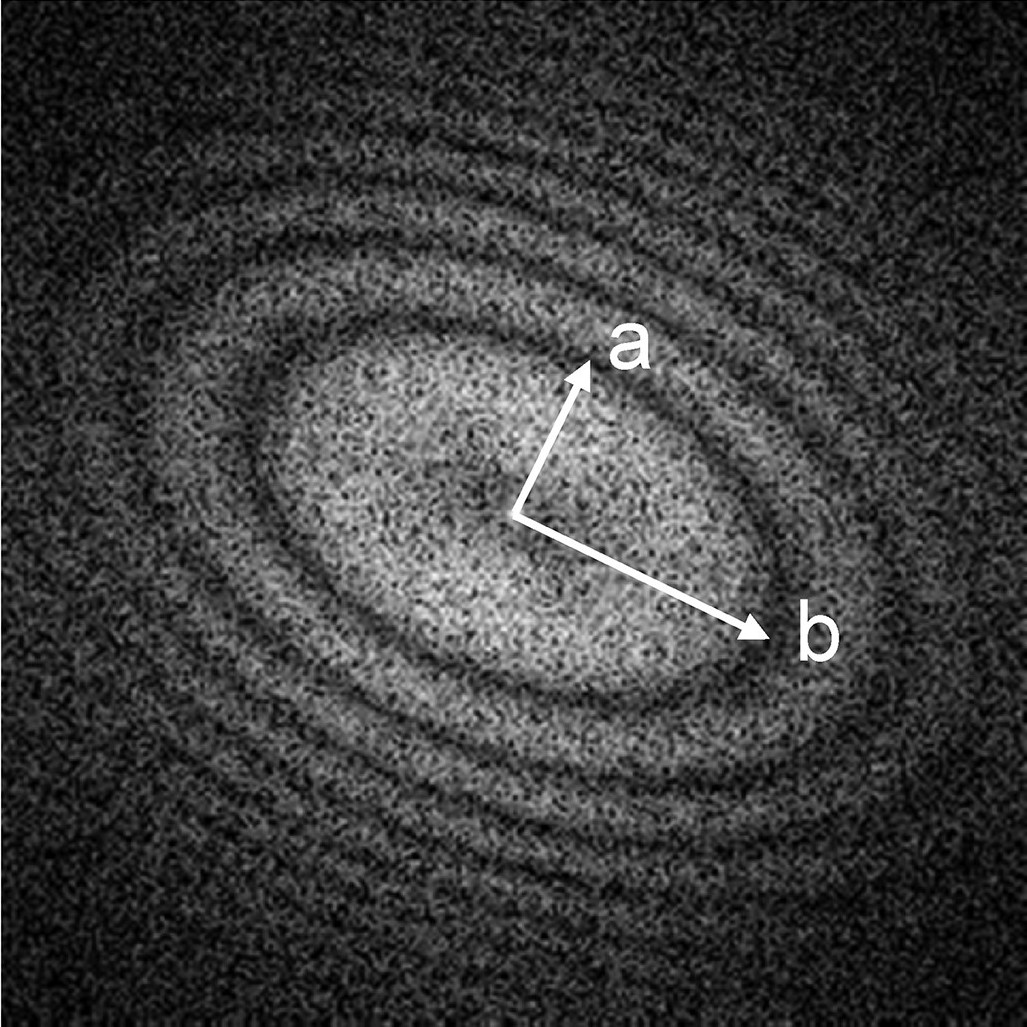
\includegraphics[width=\textwidth]{SPA/ctf/psd_as}
        \caption{Micrograph PSD with astigmatism}
        \label{fig:2:ctf:psd_as}
    \end{subfigure}\\
    Images obtained from: \cite{cryoem101}
    \caption{CTF examples}
    \label{fig:2:ctf}
\end{figure}

This \gls{ctf} is different for each micrograph and it needs to be known by later steps. Moreover, it can be used to assess the quality of the micrographs\cite{cryoem101}. The characterisation of the \gls{ctf} is accomplished by calculating the \gls{psd} of the micrograph and fitting a template onto it.

\subsection{Particle picking}
In the context of \gls{spa}, the term particle refers to the individual projections of the specimen under study. As stated earlier, a micrograph may contain many particles. Particle picking consists in pin-pointing individual particles in a micrograph. This enables extracting them to individual images in order to continue with the processing. This used to be a manual task for biologists, but recent leaps in \gls{ml} have enabled the possibility of using supervised \gls{ml} algorithms to automate this process. An example of a picking is shown in the Figure \ref{fig:2:picking}

\begin{figure}[htbp]
    \centering
    \begin{subfigure}[b]{0.45\textwidth}
         \centering
         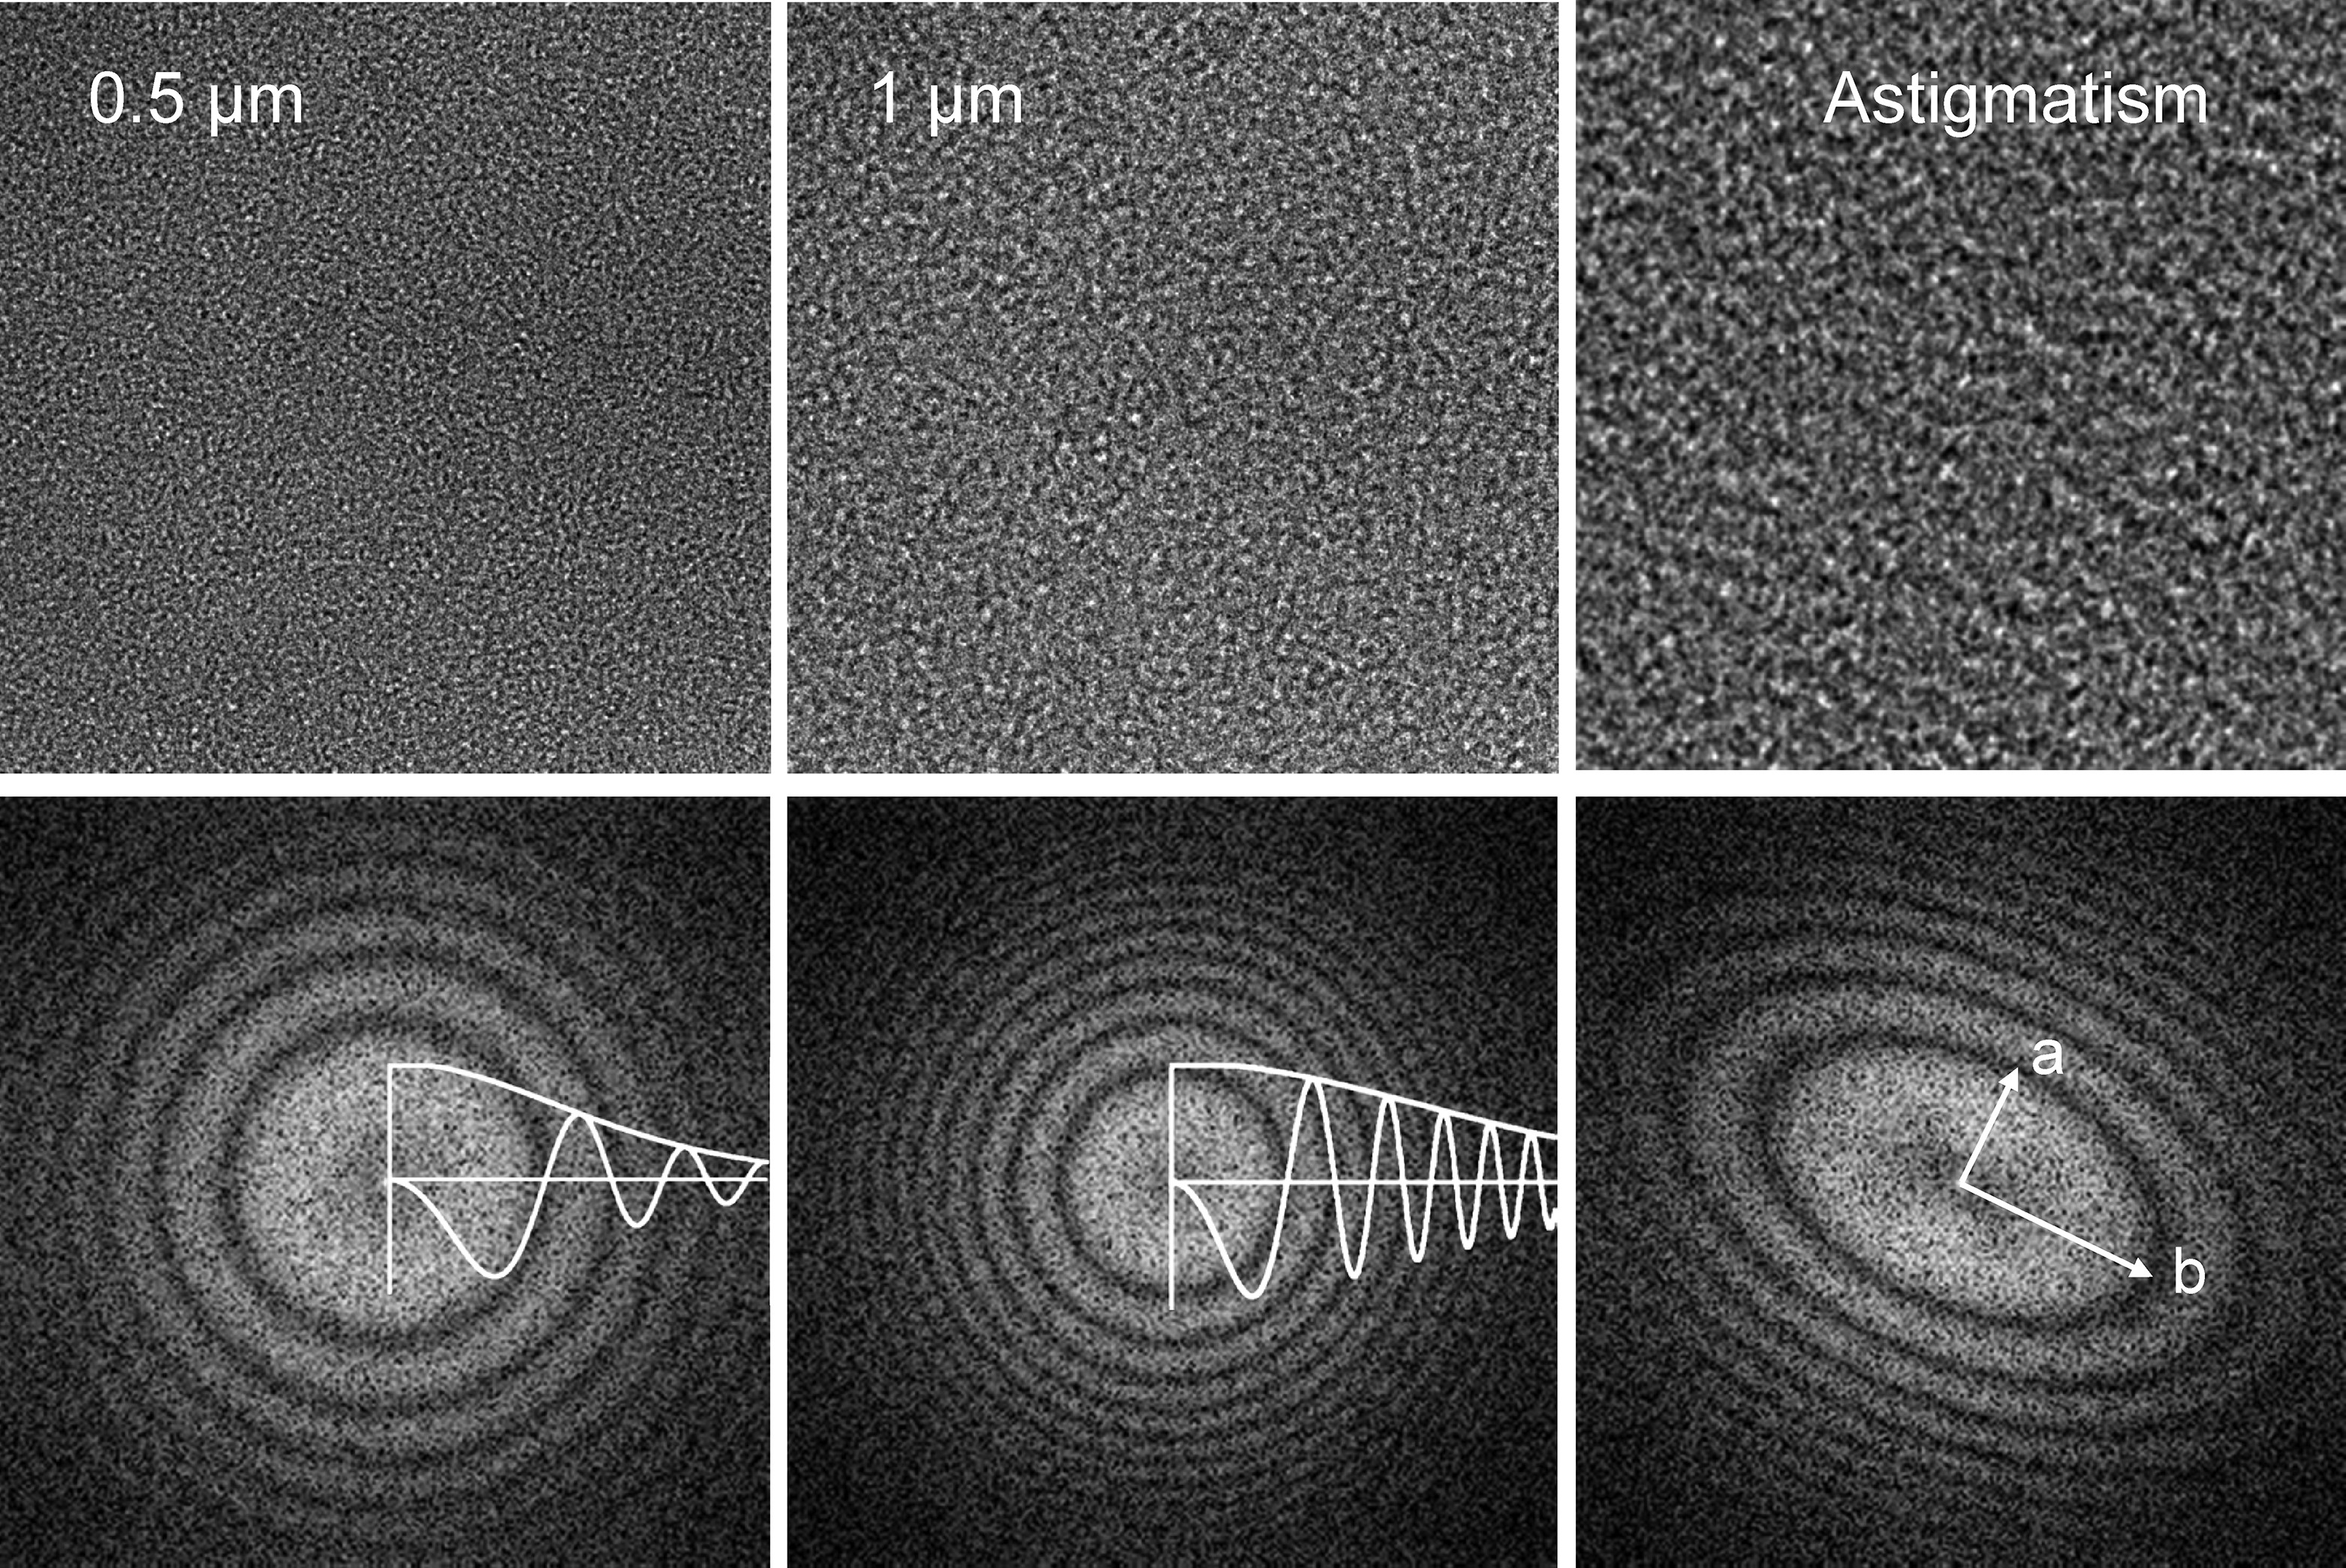
\includegraphics[width=\textwidth]{SPA/picking/original}
         \caption{Original micrograph}
         \label{fig:2:picking:original}
    \end{subfigure}
    \begin{subfigure}[b]{0.45\textwidth}
         \centering
         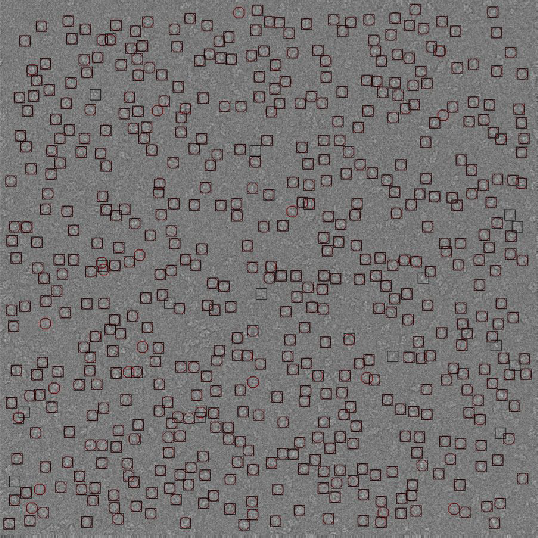
\includegraphics[width=\textwidth]{SPA/picking/picked}
         \caption{Picked micrograph}
         \label{fig:2:picking:picked}
    \end{subfigure}
    \caption{Example of a picked micrograph}
    \label{fig:2:picking}
\end{figure}

\subsection{2D Classification}
2D classification consists in comparing particles to one another and clustering similar ones. These comparisons take into consideration in-plane transforms (rotations and shifts) of the particles. Therefore, clusters are invariant to translation and rotation. These clusters are averaged so that the highly correlated parts of the particles remain intact, while uncorrelated parts -noise- are attenuated, potentially increasing the \gls{snr}. Moreover, as many micrographs with unique \glspl{ctf} are used, the missing information in the zeros of the \gls{ctf} tends to cancel out. A example of this process is illustrated in the Figure \ref{fig:2:2d_classification}.

These 2D classes have many applications. For instance, their averages can be used as a feedback to re-enforce the picking algorithm. Additionally, the lack of clusters can be used as an evidence of preferential orientations of the specimen. Similarly, poorly detailed clusters may indicate that particles belonging to them are invalid. Last but not least, these 2D classes may be used as input for downstream steps.

\begin{figure}[htbp]
    \centering
    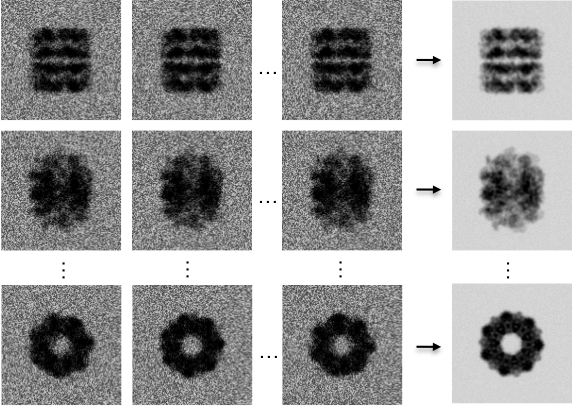
\includegraphics[width=.75\textwidth]{SPA/2d_classification}\\
    Image obtained from: \cite{greg}
    \caption{Example of 2D classification}
    \label{fig:2:2d_classification}
\end{figure}

\subsection{Ab-initio map reconstruction}
3D reconstruction is usually a \gls{sgd} algorithm which iteratively improves a 3D electron density map of the protein under study. Therefore, choosing a good starting point is important to improve the performance of the \gls{sgd} algorithm and avoid local minimums as much as possible. This starting point is known as the initial model. As the gradient descent starts at this volume, the final result will be heavily biased by it\cite{sigworth2015}.

The problem of obtaining a initial volume lies in deducing a 3D volume from a set of 2D projections that were done across unknown directions. There is a large set of approaches to address this problem. Some approaches perform a random angular assignments and then start the gradient descent from it. Some other algorithms rely on correlating a vast amount of random reconstructions\cite{vargas2014}. Finally, there are some novel approaches that make use of unsupervised \gls{ml} methods to learn a map from the particles\cite{levy2022}.

\subsection{3D Classification}
Until this point we have assumed that all particles belong to the same structure. However, this is not true in many cases, as proteins may be flexible or they might have a ligand attached to them. Figure \ref{fig:2:30s_yjeq} exhibits a protein with conformational heterogeneity due to a drug binding. If this specimen was to be captured, some particles would contain the part highlighted in orange and some others would not.

\begin{figure}[htbp]
    \centering
    \begin{subfigure}[b]{0.3\textwidth}
         \centering
         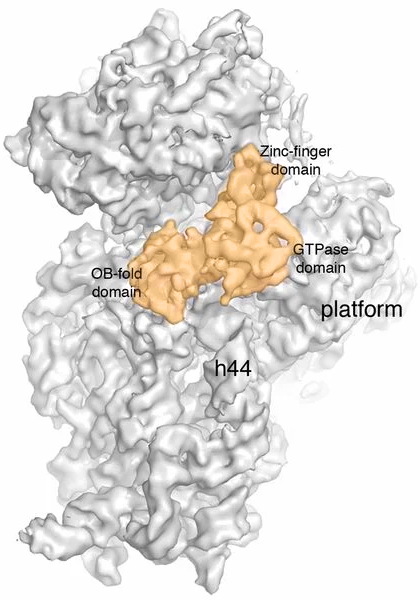
\includegraphics[width=\textwidth]{SPA/30S_YjeQ/front}
         \caption{Front view}
         \label{fig:2:30s_yjeq:front}
    \end{subfigure}
    \begin{subfigure}[b]{0.3\textwidth}
         \centering
         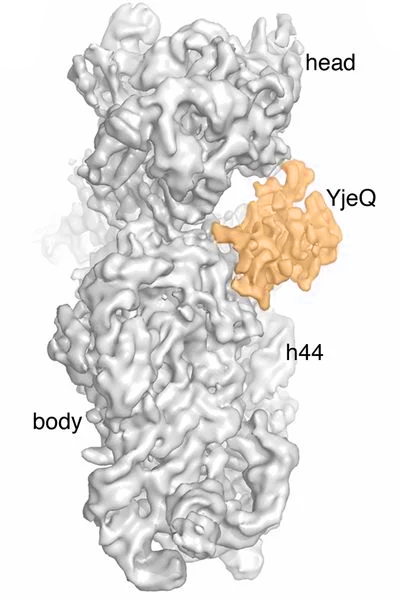
\includegraphics[width=\textwidth]{SPA/30S_YjeQ/side}
         \caption{Side view}
         \label{fig:2:30s_yjeq:side}
    \end{subfigure}\\
    Images obtained from: \cite{razi2017}
    \caption{30S ribosome with a binding}
    \label{fig:2:30s_yjeq}
\end{figure}

3D classification consists in clustering particles based on the structure they belong to. Obviously, when the input data has no conformational heterogeneity, this step is skipped.

Usually, the differences between the considered variations of the structure are very subtle, so this is not an algorithmically easy task. Some software packages perform this task in the refinement step, in a process known as multi-reference refinement.

\subsection{Refinement}
The refinement step is used to obtain a high resolution 3D electron density map of the protein under study. As stated earlier, sometimes more than one map may be desired. 

Most of the state-of-the art packages perform the following refinement cycle repeatedly. In essence, the algorithm tries to maximise the compatibility between the reconstructed volume and the experimental data. For that, it attempts to reproduce the experimental data from the reconstructed volume. This cycle is displayed in the Figure \ref{fig:2:refinement}.

\begin{enumerate}
    \item Project the current volume(s) from different angles to obtain a projection gallery.
    \item For each experimental image find the most similar image in the gallery and assign its projection angle. Note that in-plane transformations (rotations and translations) need to be taken into account. Most of the existing solutions differ in this step, as many similarity metrics and exploration patterns can be used.
    \item Reconstruct the volume(s) with the angular assigned experimental images.
    \item Repeat steps 1 to 3 using the newly obtained volume. The algorithm should converge to a local minima\cite{sigworth2015}. When the loop stops producing significant changes or a desired resolution is achieved, the cycle should be stopped.
\end{enumerate}

\begin{figure}[htbp]
    \centering
    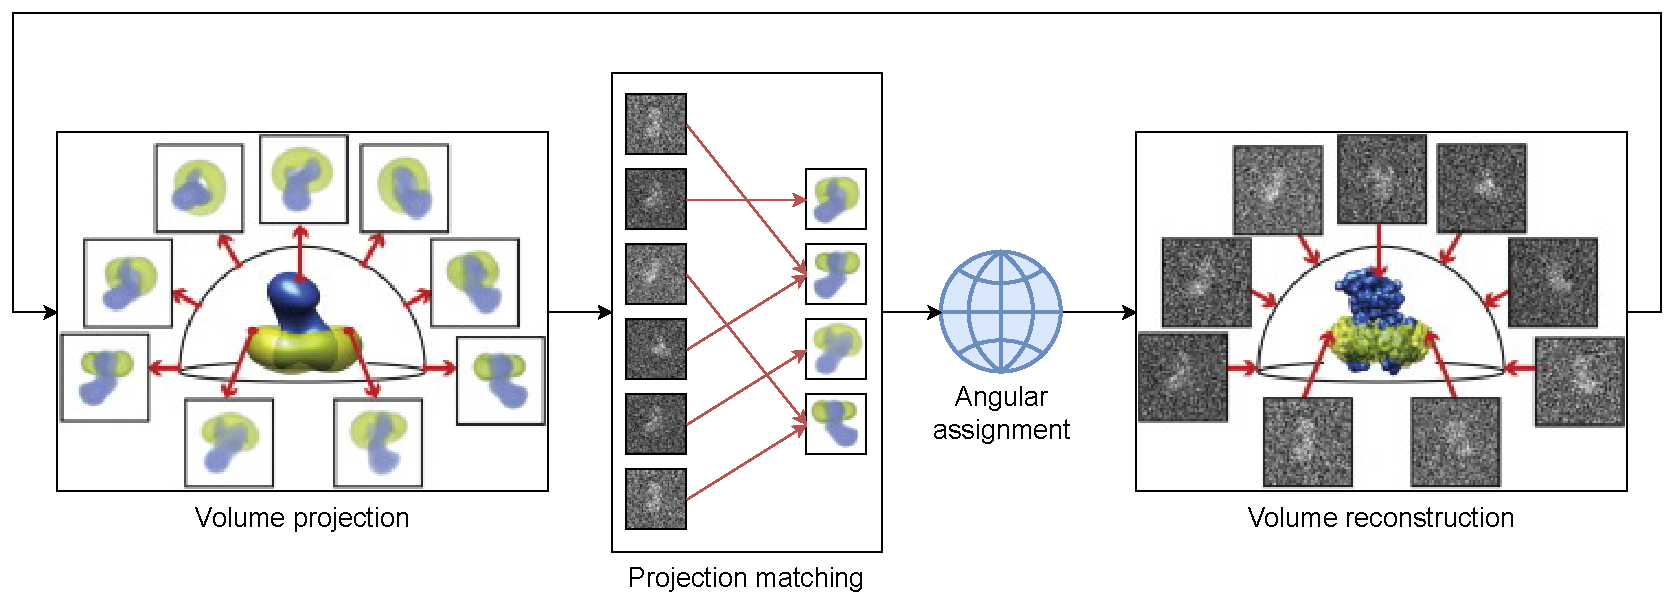
\includegraphics[width=\textwidth]{SPA/refinement}\\
    Diagram figures from: \cite{nogales2015}
    \caption{Typical refinement cycle}
    \label{fig:2:refinement}
\end{figure}

Nowadays, most implementations make use of the Fourier Central Slice theorem to perform steps 1 and 3. This theorem states that projecting a $N$-dimensional function to $N-1$ dimensions and then taking its \gls{ft} is equivalent to computing the $N$-dimensional \gls{ft} and then extracting the central hyperplane normal to the projection direction. This equivalence is shown in the Figure \ref{fig:2:3dfourier}. Most reconstruction algorithms leverage this fact by filling 3D Fourier space with appropriately oriented 2D \glspl{ft} of the particles and then taking its \gls{ift}.

\begin{figure}[htbp]
    \centering
    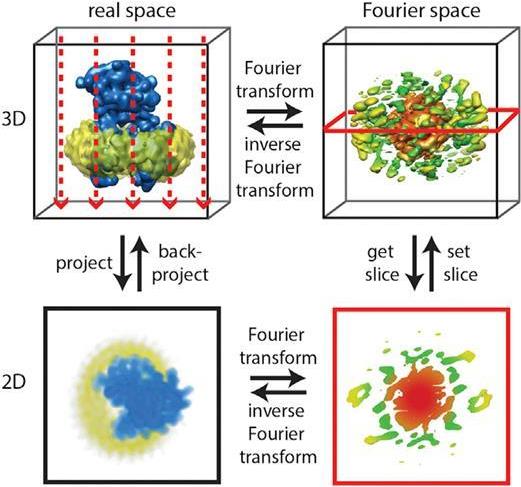
\includegraphics[width=.5\textwidth]{SPA/3d_fourier_reconstruction}\\
    Image obtained from: \cite{nogales2015}
    \caption{Fourier Slice Theorem illustration for 3D}
    \label{fig:2:3dfourier}
\end{figure}

In essence, using the Figure \ref{fig:2:3dfourier} as an example, our goal is to obtain the 3D volume in real space (top left image), but the microscope provides a collection of 2D projections of it (lower left image). Although the direct approach would be the back-projection, following the Fourier path leads to faster results. This speed improvement is largely due to the \gls{fft} algorithm.

\subsection{Model building}
The final step in \gls{spa} consists in deducing the atomic structure of the protein under study. This is a labour intensive task where a biologist needs to fit an amino acid sequence into the newly reconstructed 3D electron density map. A example of this process is displayed in the Figure \ref{fig:2:model_building}

\begin{figure}[htbp]
    \centering
    \begin{subfigure}[b]{0.3\textwidth}
         \centering
         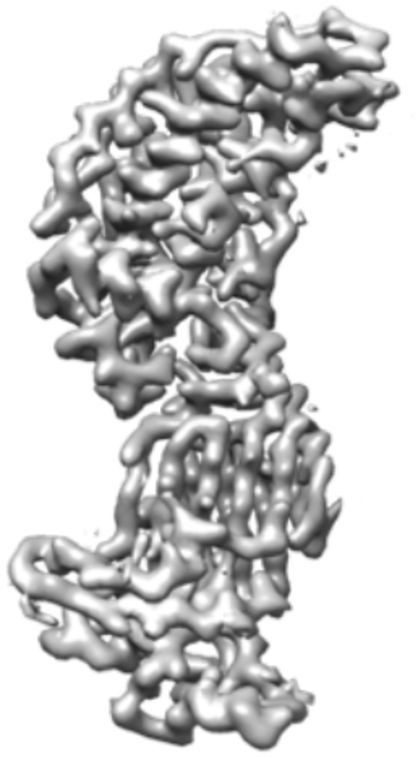
\includegraphics[width=\textwidth]{SPA/model_building/map}
         \caption{3D electron density map}
         \label{fig:2:model_building:map}
    \end{subfigure}
    \begin{subfigure}[b]{0.3\textwidth}
         \centering
         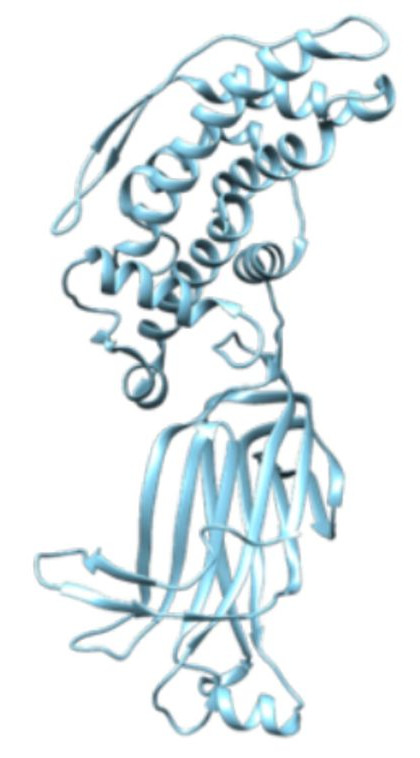
\includegraphics[width=\textwidth]{SPA/model_building/model}
         \caption{Solved structure}
         \label{fig:2:model_building:model}
    \end{subfigure}\\
    Images obtained from: \cite{pfab2020}
    \caption{Example of model building}
    \label{fig:2:model_building}
\end{figure}


\section{Conclusions}
The complexity of the \gls{spa} image processing can not be overstated. The starting point is a vast amount of data representing thousands of random projections of the specimen under study. This data is heavily contaminated with various sources of noise and other artefacts. Moreover, most of the parameters, including the projection directions, are unknown. Many times we can not even affirm that all projections belong to the same structure. All these unknowns need to be estimated from the data before attempting to perform a reconstruction. At the end, the atomic model of the protein can be deduced from this reconstruction. 

However, the effort required to obtain these atomic models is highly justified. These models give researchers a lot of knowledge and power to develop new drugs and vaccines.

\end{document}
 